\documentclass[Rapport/Rapport_main.tex]{subfiles}
\begin{document}
\subsection{CupLight}\label{sec:rap_cup_light}
I dette afsnit beskrives de design valg, der er gjort angående lyset i en CupHolder og controlleren dertil, samt hvordan de er implementeret. Til sidst laves der også en test for modulet. Dette modul anvendes udelukkende af GameController-klassen på PSoC playerside.
\subsubsection{Hardware Design}
\textbf{Lys på CupHolder}
Den overordnede hardware for koppen kan deles op i 2 dele. En del der høre til på CupHolder og et controller-kredsløb der anvendes til at styre lyset.\\
På CupHolder er det fysiske lys placeret. Det fysiske lys må ikke fylde meget og heller ikke være dyrt, da det skal passe i forhold til antallet af lys på og målene for en CupHolder, der kan ses i bilag \textbf{Kravspecifikation} i afsnit \fullref{kravspec:sec:ikke_funktionelle_krav}. Det besluttes derfor at der anvendes en common-cathode RGB-led med en diameter på 3mm \cite{RGBledDatasheet}. Grunden til at lige netop almindelige RGB-LED'er vælges over f.eks. addresserbare RGB-led'er (Eller andre led'er med indbygget chip) er for det første prisen og for det andet, så er der ikke et krav om at de enkelte LED'er på hver kopholder skal lyse individuelt.\\
RGB-LED'erne skal have for-modstande til de ben der anvendes til at styre farverne, samt 3 transistorer\cite{datasheet_bc557b} til at tænde for benene efter behov. Designet af lyset på CupHolder kan ses i figur \ref{fig:rap_cupholder_light}.
\begin{figure}[H]
    \centering
    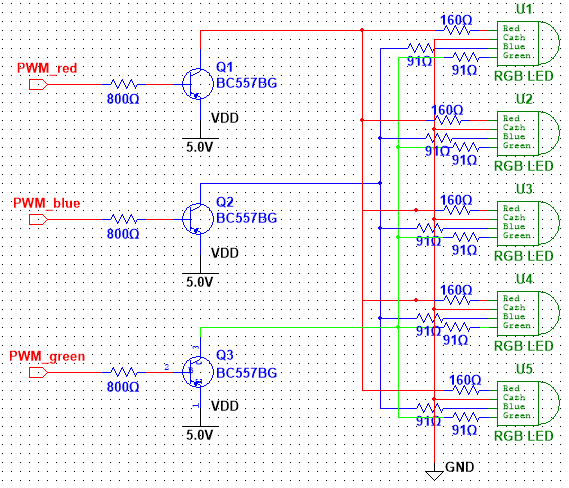
\includegraphics[width=0.9\textwidth]{HardwareDesign/CupLight/graphics/CupHolder_HW.png}
    \caption{Design af CupLight på Cupholder}
    \label{fig:rap_cupholder_light}
\end{figure}
\textbf{Controller-kredsløb til CupLight}
Kredsløbet der skal kontrollere lyset i CupHolders, skal have en egenskab, hvilket er at den skal kunne lave PWM-signaler nok til alle CupHolders. Det vil altså sige, der skal laves en controller, der kan lave 18 PWM-signaler, da den røde,grønne og blå farve skal kunne kontrolleres på alle 6 CupHolders. Løsningen skal også være billig og forholdsvis intuitiv at anvende.\\
CupLight controller-kredsløbet laves af 3 74HC595 skifteregistre\cite{datasheet_shiftreg}, hvor der kan laves et PWM signal på deres output ben ved at styre registrene gennem SPI-kommunikation. På denne måde er man med 3 registre i stand til at lave 24 individuelle PWM-signaler, hvilket kan forbindes til de forskellige transistorer i CupHolders. Designet af controlleren for lyset kan ses i figur \ref{fig:rap_cuplight_controller}.
\begin{figure}[H]
    \centering
    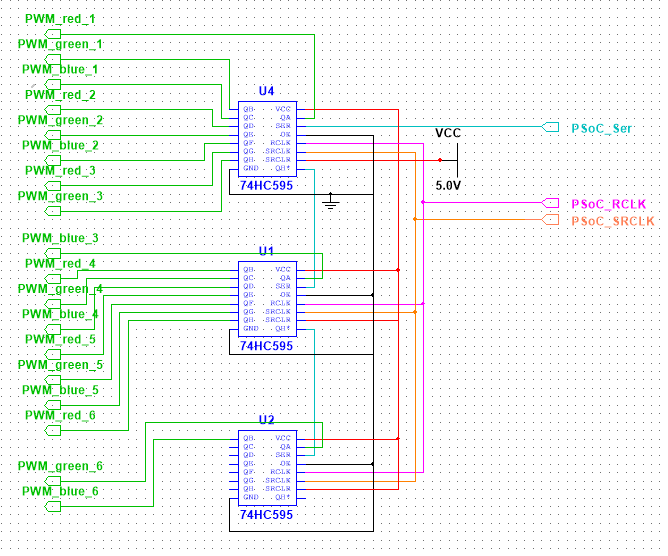
\includegraphics[width=0.9\textwidth]{HardwareDesign/CupLight/graphics/CupLight_HW_Controller.png}
    \caption{Design af controller for CupLight}
    \label{fig:rap_cuplight_controller}
\end{figure}
Hardwaredesignet er videre udspecificeret i dokumentet \textbf{Hardware Design} i afsnit \fullref{hwdesign:sec:sec:cuplight_hw_design}.
\subsubsection{Software Design}
Til lyset skal der laves kode til at styre CupLight-controller hardwaren. Det vil altså siges, at der skal laves software, der ved SPI-kommunikation kan kontrollere et skifteregister til at lave det ønskede PWM-signal på en given output pin. Til dette skal der anvendes et timer-interrupt, der bestemmer hvornår skifteregisteret skal opdateres med nye værdier. Der laves desuden et klasse diagram for dette lille interface, der kan ses på figur \ref{fig:rap_cd_cuplight}.
\begin{figure}[H]
    \centering
    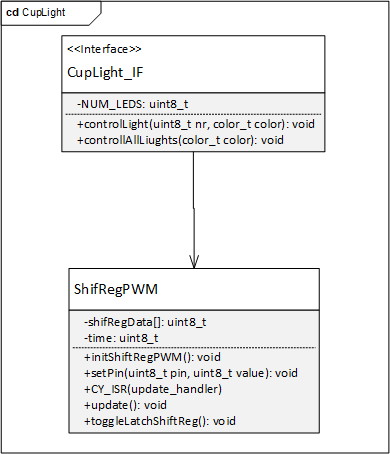
\includegraphics[width=0.5\textwidth]{Softwaredesign/CupLight_IF/graphics/CD_CupLight.png}
    \caption{Klassediagram for CupLight modulet}
    \label{fig:rap_cd_cuplight}
\end{figure}
Alt Software design er udspecificeret mere i \textbf{Software Design} dokumentet i afsnit \fullref{swdesign:sec:cuplight_sw_design}.
\subsubsection{Implementering}
Implementeringen af CupLight\_IF er lavet i IDE'et PSoC-creator 4.2. Det er implementeret ved moduler bestående af header- og source-filer. Til implementeringen af \textsc{ShiftRegPWM} er der hentet inspiration fra Timo Denk's blog\cite{shiftregpwm}. De vigtigste funktioner og detaljer i implementeringen kan ses i dokumentet SoftwareDesign i afsnit \fullref{swdesign:sec:cuplight_sw_impl}.
\subsubsection{Modultest}
Til test af CupLight modulet blev der anvendt et UART-komponent på PSoC'en til at sætte forskellige PWM værdier. PSoC'ens SPI-kommunikation blev forbundet til et 74HC595 skifteregister, og på output pins af dette register blev der så målt på de forskellige PWM-signaler. Der blev målt rise-time af PWM-signalet, samt nøjagtigheden af PWM-signalet i forhold til det ønskede. Senere forbandtes controller-kredsløbet til en LED for at teste at farverne også stemte overens med det forventede. Resultaterne fra modultesten kan ses i dokumentet \textbf{Modultest} i afsnit \fullref{modultest:sec:cuplight_test}.\\\\
Konklusionen af modultesten er, at controller modulet er i stand til at generere tilstrækkeligt præcise PWM-signaler til at kunne styre RGB-led'er til mere end 10 forskellige farver. 
\end{document}